\chapter{Algae canal}
%

% - Purpose & Problem description:
%     These first two parts give reader short details about the test case,
%     the physical phenomena involved and specify how the numerical solution will be validated

\section{Purpose}

This test case validates the algae transport module in \telemac2d, and it is a useful example for a user
wanting to see how to make use of the particle positions and velocities. In addition, there is a python
script (\texttt{ConvertDat2Vtu.py}), added to this test case which can be used to convert the particle
result file from a Tecplot format to a ParaView format.

\section{Description}

To validate the algae bloom transport model the experiment presented in \citet{Joly_these} and \citet{Joly_jhr}
will be modelled. More validation of the theory can also be found in \citet{Joly_pof}. The flow configuration
of this experiment is that of partially obstructed open flat bed channel flow, which has the advantage of
generating a large recirculation pattern downstream of the obstructing groyne. In this experiment a fluid with
a density of $1000$ kg/m$^{3}$ and a flow rate of $0.5$ m/s was imposed in a $2$ m wide channel which was
obstructed by a groyne $0.5$ m long and $0.1$ m thick. The water depth was imposed to be $0.3$ m before the flow
arrived at the groyne. The groyne was constructed high enough to stop overtopping. The experimental setup is
described in figure~\ref{fig:exp_setup}, and the Reynolds number was thus $10^{6}$.

\begin{figure}[hb]%
\begin{center}
%
  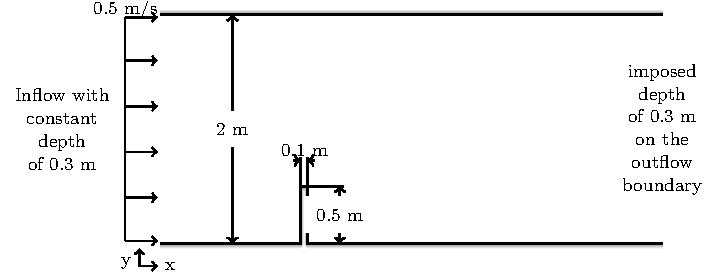
\includegraphics[width=0.75\textwidth]{./Figures/CanalAlgExpSetup}
%
\end{center}
\caption{Experimental setup for a partially obstructed flat bed open channel flow (top view). In this experminent
spherical particles were released to validate the algae transport of Telemac-2D.}
\label{fig:exp_setup}
\end{figure}

The flow velocities are well modelled using Telemac-2D. In this case the flow is modelled using a $k$-$\varepsilon$
closure and it is validated against experimental measurements and another simulation performed with OpenFoam, which
solves the two-dimensional Navier-Stokes equations with a $k$-$\varepsilon$ closure using a finite volumes method
\citep{OpenFoam}. The horizontal fluid velocities are presented in figure~\ref{fig:profil_vitesses_canal}.

\begin{figure}[H]%
\begin{center}
%
  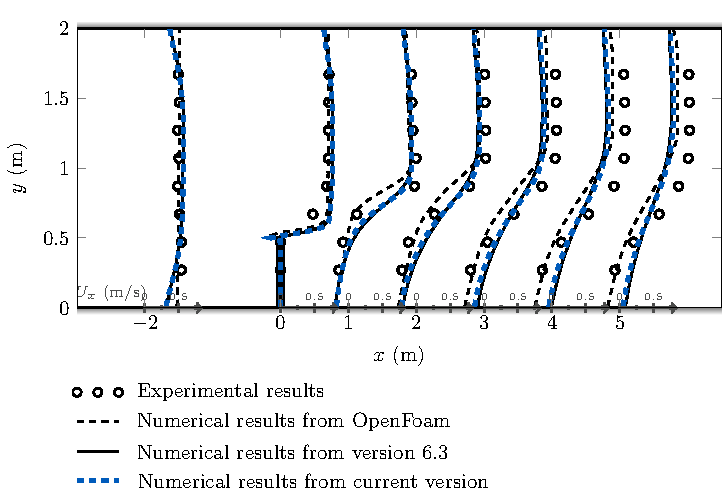
\includegraphics[width=0.75\textwidth]{./Figures/CanalAlgFluidVelocities}
%
\end{center}
\caption{Profiles of the horizontal velocity plotted at different locations along the canal. The small axis marked on
top of the x-axis represent the values of velocity magnitude.}
\label{fig:profil_vitesses_canal}
\end{figure}

Spheres $6$ mm in diameter ($D_s$) and of density $\rho_s=2200$ kg$\cdot$m$^{-3}$ were released in the flow one at a
time at fixed intervals (about $1$ Hz). This was done to ensure that particles would not affect each other's motion.
Several particles were released at different positions in the flow and the trajectories for these particles were
recorded at different locations. The trajectories of these particles were measured with a camera that was placed above
the flow so that the position of particles entering a window of measurement were recorded, see
figure~\ref{fig:exp_setup2}. The process used to extract the trajectories is presented in \citet{Joly_these}.

\begin{figure}[H]%
\begin{center}
%
  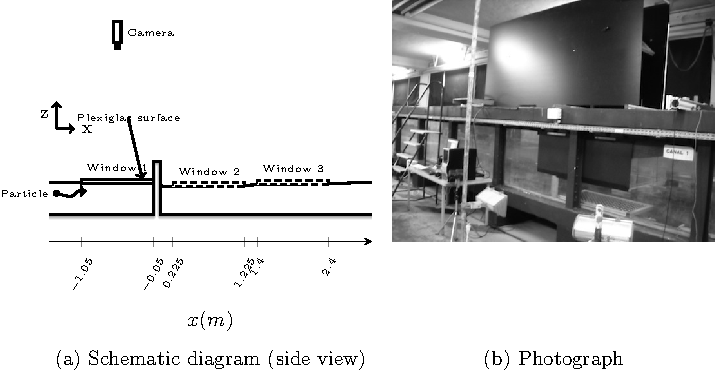
\includegraphics[]{./Figures/CanalAlgExpSetup2}
%
\end{center}
\caption{Experimental setup to record the particle trajectories.}
\label{fig:exp_setup2}
\end{figure}



% - Numerical parameters:
%     This part is used to specify the numerical parameters used
%     (adaptive time step, mass-lumping when necessary...)
%
%
\subsection{Geometry and mesh}

The mesh consist of the mesh has $36\,996$ nodes and $73\,346$ elements.
The mesh elements size was about $0.1$ m at the inflow, $0.015$ m around the groyne and $0.3$ m at the
outflow. A picture of the mesh can be found in figure~\ref{fig:mesh_obstruc_channel}.

\begin{figure}[H]%
\begin{center}
%
  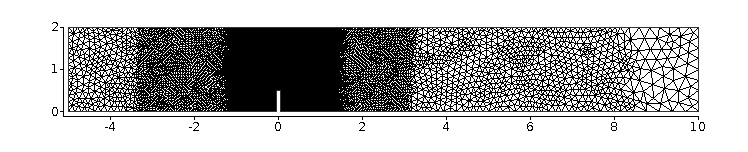
\includegraphics[width=0.85\linewidth]{./Figures/Images/mesh_obstruc_channel}
%
\end{center}
\caption{Mesh used to simulate the obstructed channel flow.}
\label{fig:mesh_obstruc_channel}
\end{figure}

\subsection{Numerical parameters}
To help the simulation run faster, the computation is continued from a previous file, i.e. using the
following keywords:

\lstset{language=TelemacCas,
        basicstyle=\scriptsize\ttfamily}

\begin{lstlisting}[frame=trBL]
COMPUTATION CONTINUED = YES
PREVIOUS COMPUTATION FILE =
'./ini_canal_algae_en.slf'
INITIAL TIME SET TO ZERO = YES
\end{lstlisting}

In the simulations $1000$ spheres will be released with diameter $0.006$ m and density $2200$ kg$\cdot$m$^{-3}$.
The following keywords activate the algae transport module and set these physical characteristics:

\lstset{language=TelemacCas,
        basicstyle=\scriptsize\ttfamily}

\begin{lstlisting}[frame=trBL]
/----------------------------------------------------------------------/
/                     ALGAE OPTIONS
/----------------------------------------------------------------------/
NUMBER OF DROGUES = 1000
PRINTOUT PERIOD FOR DROGUES = 40
DROGUES FILE = './alg_pos.dat'
ALGAE TRANSPORT MODEL = YES
DIAMETER OF ALGAE = 0.006
DENSITY OF ALGAE = 2200.0
ALGAE TYPE = 1
\end{lstlisting}


Finally, the particle defined by editing the user subroutine \texttt{flot.f}, and adding these lines of code:

\lstset{language=Fortran,
        basicstyle=\scriptsize\ttfamily}

\begin{lstlisting}[frame=trBL]
      IF(LT.EQ.ALGAE_START) THEN
        DO I=1,NFLOT_MAX
          CALL ADD_PARTICLE(0.175D0,0.45D0,0.D0,I,NFLOT,
     &                    NFLOT_MAX,XFLOT,YFLOT,YFLOT,TAGFLO,
     &                    SHPFLO,SHPFLO,ELTFLO,ELTFLO,MESH,1,
     &                    0.D0,0.D0,0.D0,0.D0,0,0)
        END DO
      ENDIF
\end{lstlisting}

%
% - Results:
%     We comment in this part the numerical results against the reference ones,
%     giving understanding keys and making assumptions when necessary.
%
%
\section{Results}

\subsection{Explantion of the results}

For this test case, the particles are released at position ($0.175$,$0.45$) and recorded using window 2
(see \figurename~\ref{fig:exp_setup2}a). More results are presented in \citet{Joly_these}.

To analyse the trajectories of the particles, the window of measurements is then divided into four quadrants.
The number of particles entering each quadrant, and the time spent inside is recorded. The values are then
non-dimensionnalised using the sum of all the quadrants, i.e.:

\begin{subequations}
\begin{align}
N_{res,Q_i}=&\frac{N_{Q_i}}{\sum_j^4{N_{Q_j}}}
\\
T_{res,Q_i}=&\frac{T_{Q_i}/\sum_j^4{T_{Q_j}}}{N_{Q_i}/\sum_j^4{N_{Q_j}}}
\end{align}
\end{subequations}

Where $N_{res,Q_i}$ and $T_{res,Q_i}$ represent the non-dimensionnalised proportion of particles and mean time
of residence inside a quadrant $Q_i$. $N_{Q_i}$ is the number of particles recorded in a quadrant and $T_{Q_i}$
is the cumulative time spend by all the particles present in this quadrant.

This method of writing the results allows a comparison between numerical and experimental results, as during the
experiment is was impossible to know if a particle that exited the window of measurement would re-enter it at a later time.

These results are plotted in figures~\ref{fig:quadrant_npart} and~\ref{fig:quadrant_tresid}, where for each quadrant the value
of interest is plotted along a line going from the inner most corner to the outter most corner. The length scales for these
values are chosen in such a way that the maximum value is placed on the outer most corner. The points plotted for each quadrant
are then linked together to form an area. An annotated description of the results is given in \figurename~\ref{fig:expe_canal_annotated_example}.

\begin{figure}[H]%
\begin{center}
%
  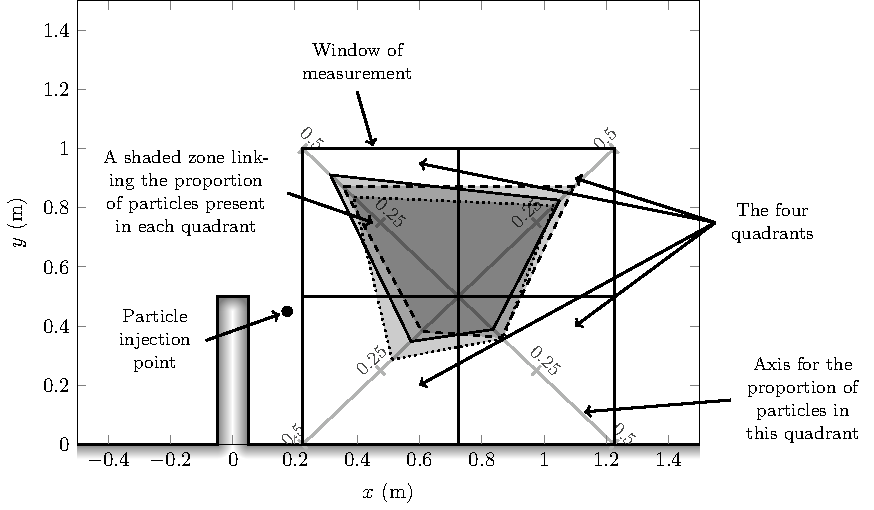
\includegraphics[]{./Figures/CanalAlgAnnotatedFigure}
%
\end{center}
\caption
{An annotated example to explain how the proportion of particles entering each quadrant of a window of measurement are presented.}
\label{fig:expe_canal_annotated_example}
\end{figure}

The velocity of the particles were also analysed. To do so, profile plots were done of the properties of the particles crossing the
line at $x=0.55$ m. These figures can be found in figures~\ref{fig:profile_x0p55_N} to~\ref{fig:profile_x0p55_V_Y}.

\subsection{Simulation results}

The first result presented will be the proportion of particles entering a quadrant and their mean time of residence. These results
will be compared to experimental results and results where the fluid velocities were simulated using OpenFoam. They are presented in
\figurename{}s~\ref{fig:quadrant_npart} and~\ref{fig:quadrant_tresid}.

\begin{figure}[H]%
\begin{center}
%
  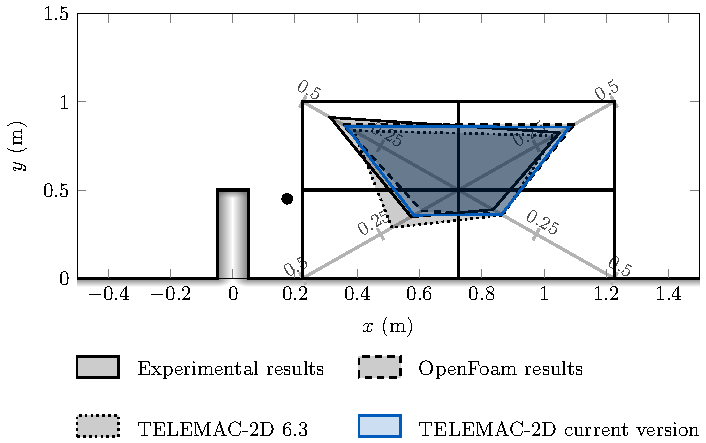
\includegraphics[]{./Figures/CanalAlgQuadrantNpart}
%
\end{center}
\caption{Partially obstructed channel flow: proportion of released particles entering a quadrant of the window of measurement.}
\label{fig:quadrant_npart}
\end{figure}

\begin{figure}[H]%
\begin{center}
%
  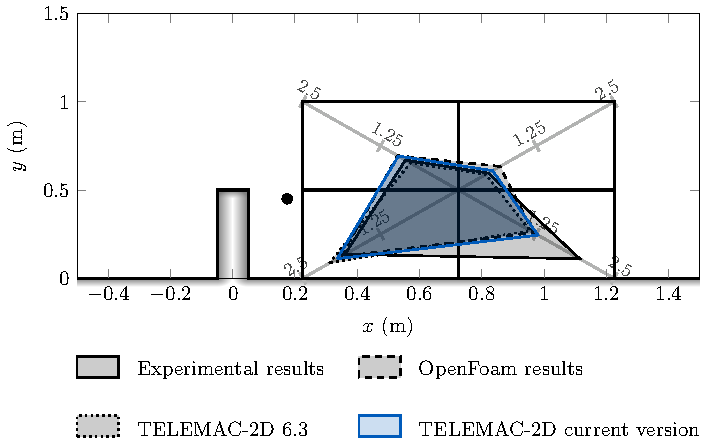
\includegraphics[]{./Figures/CanalAlgQuadrantTrsd}
%
\end{center}
\caption{Partially obstructed channel flow: mean particles residence time inside a quadrant of the window of measurement.}
\label{fig:quadrant_tresid}
\end{figure}

As can be seen from \figurename{}s~\ref{fig:quadrant_npart} and~\ref{fig:quadrant_tresid} the \texttt{ALGAE\_TRANSP} module of
Telemac-2D models accurately the position of spherical particles. There is only the mean time of residence of the bottom right
corner which has noticeable differences, but this is also the case with the fluid velocities model using OpenFoam. This would
suggest that the center of the recirculation pattern might be a bit off when modelled in Telemac-2D.

The next results will assess the ability of the model to predict the velocities of the particles released in the flow. In
\figurename{}s~\ref{fig:profile_x0p55_N} to~\ref{fig:profile_x0p55_V_Y} profiles will be shown of the fraction of particles
crossing the section defined by $x=0.55$ m, as well as the horizontal and vertical velocities ($V_x$ and $V_y$).

\begin{figure}[h!]%
\begin{center}
%
  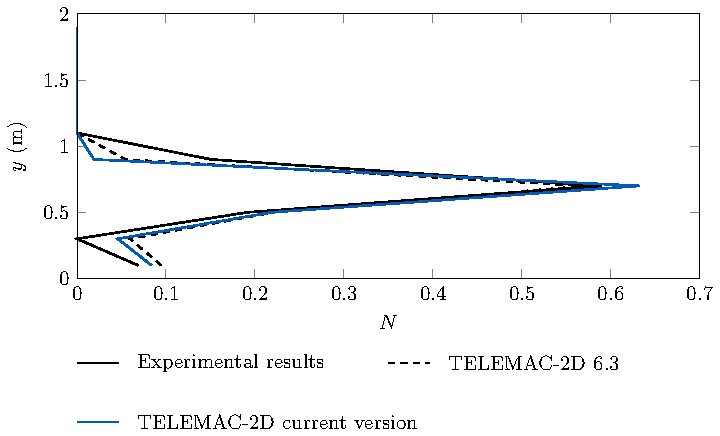
\includegraphics[]{./Figures/CanalAlgProfile_x0p55_N}
%
\end{center}
\caption{Partially obstructed channel flow: fraction of particles crossing the section defined by $x=0.55$ m.}
\label{fig:profile_x0p55_N}
\end{figure}

\begin{figure}[h!]%
\begin{center}
%
  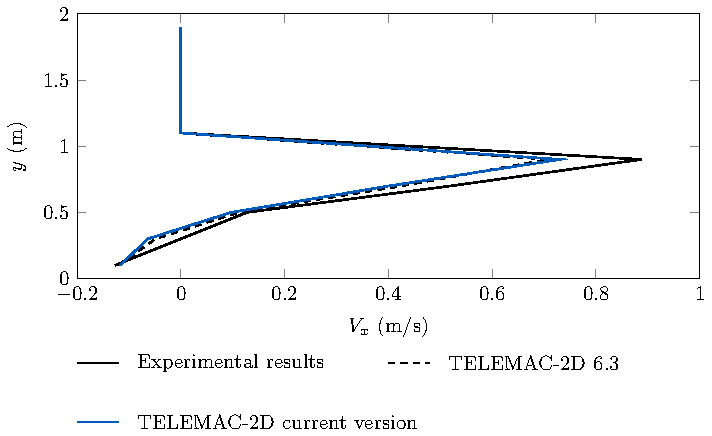
\includegraphics[]{./Figures/CanalAlgProfile_x0p55_Vx}
%
\end{center}
\caption{Partially obstructed channel flow: velocity along x-axis of particles crossing the section defined by $x=0.55$ m.}
\label{fig:profile_x0p55_V_X}
\end{figure}

\begin{figure}[h!]%
\begin{center}
%
  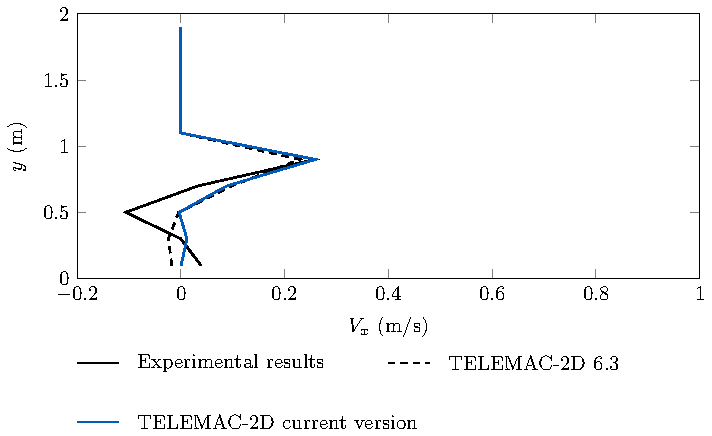
\includegraphics[]{./Figures/CanalAlgProfile_x0p55_Vy}
%
\end{center}
\caption
{Partially obstructed channel flow: velocity along y-axis of particles crossing the section defined by $x=0.55$ m.}
\label{fig:profile_x0p55_V_Y}
\end{figure}

The results presented in figures~\ref{fig:profile_x0p55_N} to~\ref{fig:profile_x0p55_V_Y} shows again that the module
\texttt{ALGAE\_TRANSP} models accurately the velocity. The only region of error would for the vertical velocity near
the solid boundaries, but this probably linked to the previous mis-estimation of the center of the recirculation
pattern in Telemac-2D. Furthermore the result are still independent of the number of processors used.

